
\section{Introducción}
El diseño, desarrollo, fabricación, armado, simulación y lanzamiento de cohetes, no es una tarea
sencilla ni repetida en intervalos de cortos de tiempo, al contrario, suelen llevar décadas y una
fuerte inversión para que sean posibles estos logros. El diseño y auge de vehículos VTVL viene
a subsanar estos factores ya que una vez terminada la misión el vehículo se puede reutilizar,
con mínimas intervenciones, y estaría listo para una nueva misión, atacando estos dos puntos principales anteriormente mencionados, el tiempo y el costo. Esto difiere del método convencional donde el vehículo, luego de completar la misión, pasa a formar parte de basura espacial o, en el mejor de los casos, es recuperado del mar como el caso del Space Shuttle. 

\medskip

El concepto de un vehículo VTVL es tan viejo como el primer alunizaje: despega verticalmente (como la mayoría de los cohetes
convencionales) y aterriza verticalmente, por sí solo sin necesidad de ser tripulado con el
objetivo de completar una misión. Esto supone una gran variante de ventajas, como ser una de
las más destacadas el reutilizamiento del vehículo, con todo lo que ello implica, logrando una
optimización de los costos, disminución de huella ecológica, y tiempo de desarrollo para las empresas interesadas. Traen en si varias ventajas frente a otros vehículos voladores como la gran reducción de espacio necesario para despegar y aterrizar. Esto no es un detalle menor dado que la mayor parte de la superficie terrestre no son pistas de aterrizaje si no más bien terreno formado naturalmente.

\medskip


\medskip

Este documento propone el diseño, simulación, control y fabricación de un vehículo con capacidades VTVL siendo un prototipo de baja escala. 
Este prototipo serviría como punta pie inicial
para vehículos de escala mayor que puedan completar misiones espaciales. Existen varias ventajas de implementar este tipo de tecnología.

\medskip

A baja escala, un vehículo que despega y aterriza por su cuenta tiene la capacidad de
superar cualquier obstáculo terrestre que se presente. Esto puede ser de gran utilidad en ambientes hostiles para el
ser humano, que esto se logre de manera rápida y efectiva podría ser la diferencia entre el
éxito o no de la misión.
Como ser el transporte de insumos médicos en tiempo real desde que un paciente lo requiere,
en zonas de acceso limitado.

\medskip

En la última década hay un interés renovado en imágenes espaciales. El vehículo podría adquirir imágenes para fines de sistemas de monitoreo y análisis geoespacial como hacen las empresas \textit{Ceres Imaging} y \textit{Satellogic}. %de una situación en la que no se disponga del tiempo suficiente para el accionar convencional a bajas velocidades como ser un helicóptero o un dron.  

\medskip

El vehículo una vez desarrollado y funcionando, puede servir de plataforma para diversos
estudios de fenómenos de dinámica de fluidos, como ser, mediciones aerodinámicas,
investigación del \textit{fuel sloshing} en vehículos con tanques esbeltos.

\medskip

Un vehículo de escala reducida provee la capacidad de testear sistemas de control. Si se pierde el vehículo ante una falla el costo total de perdidas seria mucho menor con respecto a un vehículo mas grande con sistemas caros y complejos. Al tener un sistema de control definido en términos de parámetros del vehículo, se puede escalar para luego ser probado en un vehículo mas grande. Siendo un sistema más chico y manipulable que el vehículo de escala grande se tornaron más fáciles las tareas de resolver los problemas software y hardware de vuelo que surgieron durante las pruebas.

\medskip


Los sistemas de vehículos orbitales tienen sistemas complejos que deben ser testeados en una primera etapa mediante algún ensayo controlado. El vehículo que se desarrolla en el presente documento podría ser usado para tales fines como una plataforma para pruebas como ser el despliegue de una nariz o etapa, comprobación de sensores y actuadores a gran velocidad y con empuje variable.

\medskip

La tecnología VTVL permite a los cohetes de SpaceX aterrizar verticalmente después de su lanzamiento, en lugar de caer en el océano o en tierra y luego ser recuperados. Esto significa que los cohetes pueden ser reutilizados para misiones futuras, lo que reduce significativamente los costos de los lanzamientos espaciales. Antes de la introducción de la tecnología VTVL, la mayoría de los cohetes eran diseñados para ser utilizados solo una vez, lo que hacía que los costos de los lanzamientos fueran mucho más altos.
La primera vez que SpaceX logró aterrizar con éxito un cohete Falcon 9 fue en diciembre de 2015, y desde entonces ha logrado muchos otros aterrizajes exitosos, tanto en plataformas en tierra como en barcos en el mar. El aterrizaje vertical de los cohetes de SpaceX es una hazaña técnica impresionante, ya que los cohetes deben desacelerar y estabilizarse en el aire antes de aterrizar de manera segura en una plataforma pequeña.


\begin{figure}[htb]
    \centering
    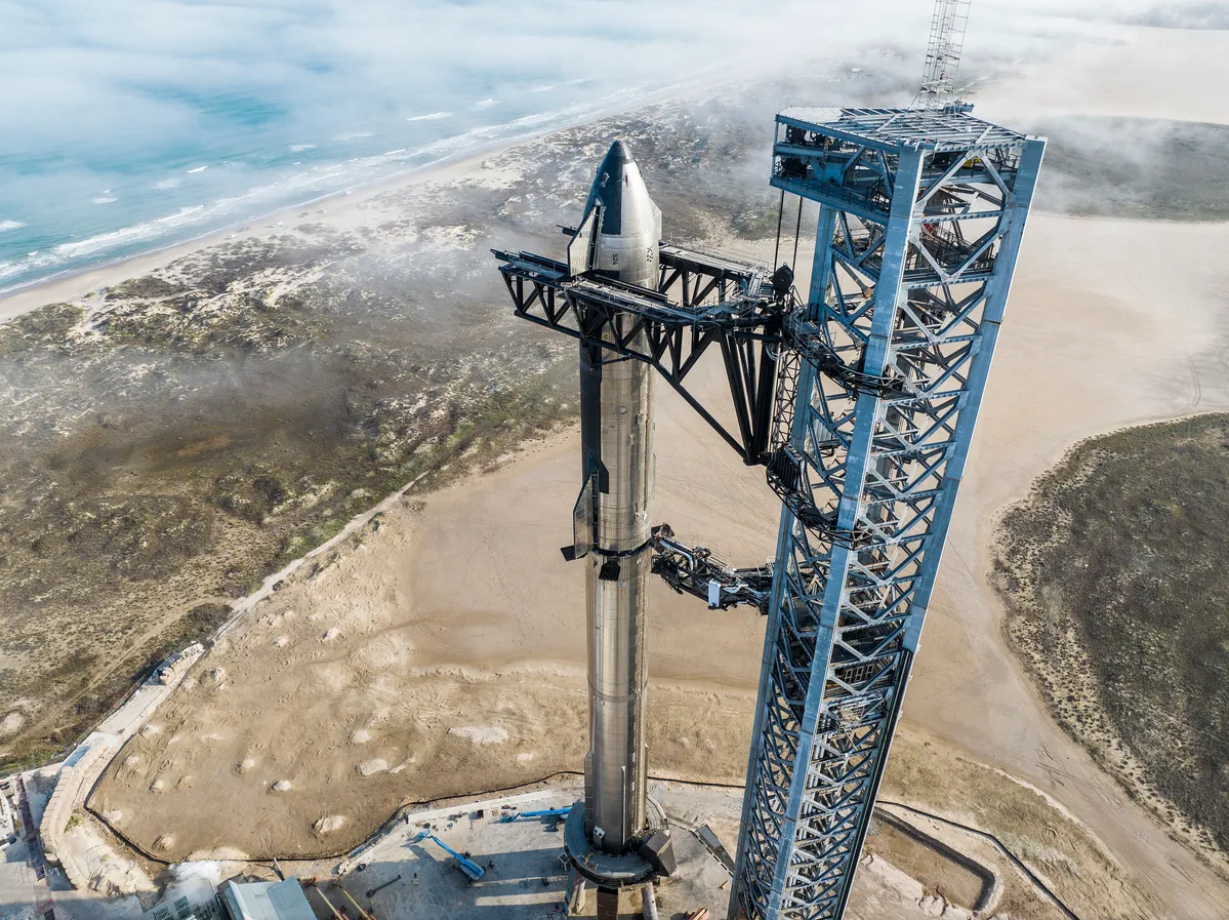
\includegraphics[width=0.8\linewidth]{fig/starhip2.png}
    \caption{Starship de SpaceX en rampa de lanzamiento.}
    \label{fig:starshipcool}
\end{figure}


Además de utilizar la tecnología VTVL en sus cohetes, SpaceX está trabajando en una nave espacial reutilizable llamada Starship, que utilizará esta tecnología para aterrizar en la Luna, Marte y otros destinos. La Starship también será capaz de realizar misiones terrestres y de corta duración, como vuelos turísticos suborbitales. La tecnología VTVL es una de las muchas innovaciones que SpaceX está utilizando para hacer que los viajes espaciales sean más asequibles y accesibles para más personas en el futuro.

\medskip

Otra organización que está apostando a la tecnología de lanzadores reutilizables es la ESA. Esta tiene un proyecto destinado a acelerar el desarrollo de tecnología de lanzadores reutilizables para las partes interesadas en el sector aeroespacial europeo. Se tiene pensado tener un lanzador reutilizable para 2030 llamado Ariane Next. Uno de los pasos a seguir antes de llegar a ese punto es el desarrollo del proyecto FROG. El proyecto FROG es un demostrador tecnológico para algoritmos de control y de métodos ágiles de proyectos \cite{rmili2019frog}. Cabe destacar que antes del FROG se pasó por una etapa preliminar de desarrollo con un vehículo con prestaciones casi idénticas al vehículo detallado en este documento. 

La ESA también ha estado trabajando en un proyecto llamado "Space Rider", que es una nave
espacial reutilizable que se lanzará al espacio en un cohete Vega-C. Una vez terminada la misión en órbita podrá volver a la tierra y aterrizar horizontalmente o verticalmente en modo VTVL. Space Rider se está diseñando como una
plataforma multipropósito para la realización de experimentos científicos y tecnológicos en órbita
terrestre baja LEO. Además, la ESA ha estado colaborando con empresas privadas europeas en el
desarrollo de cohetes reutilizables que utilizan este tipo de tecnologías. Como la empresa alemana Isar
Aerospace que está trabajando en el desarrollo de un cohete de lanzamiento de satélites reutilizable.

\begin{figure}[htb]
    \centering
    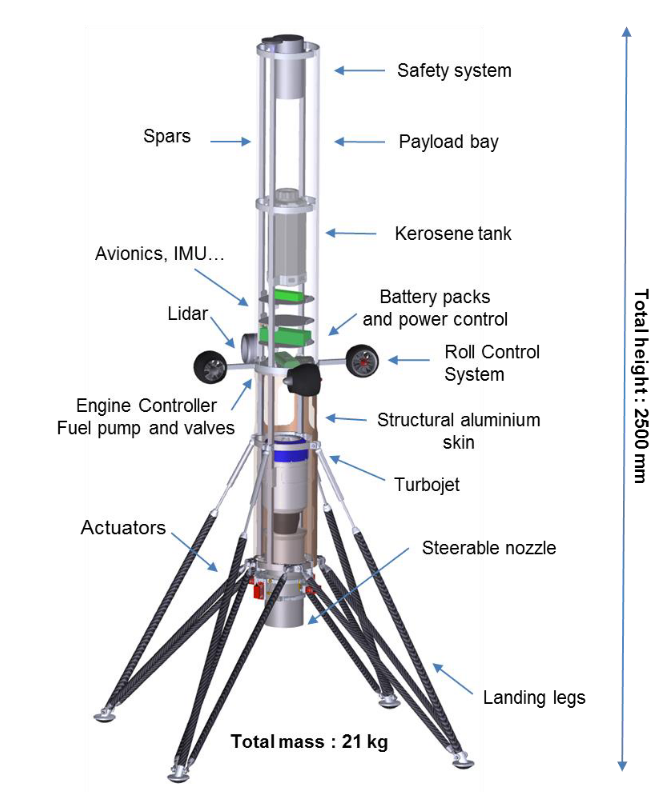
\includegraphics[width=0.8\linewidth]{fig/frogTArch.png}
    \caption{Arquitectura de FROG-T de la ESA \cite{rmili2019frog}.}
    \label{fig:frogtarch}
\end{figure}

\null\newpage
\clearpage

\section{Estudios}
En lo que se refiere a la construcción del vehículo, el diseño propuesto paso por varias etapas y
decisiones de ingeniería hasta su forma final. Desde su diseño en lápiz y papel hasta la
simulación del CAD con el detalle del ultimo bulón del ensamble para ser cargado al sistema de control en la forma de una matriz de inercia, centro de masa y dinámicas de vuelo, e ir en paralelo retroalimentándose con estos parámetros. En base a esto se realizaron modificaciones sobre el código de control y las simulaciones.


\subsection{Agua como propelente}\label{ssec:propAgua}
El primer prototipo muy distante del diseño final perteneciente a este trabajo, consistía en un
recipiente a presión con agua, abulonado a un chasis, con un cardán y actuadores para poder redirigir el
empuje. 

\medskip

La figura~\ref{fig:bottlerocket} muestra los resultados de una simulación de un vehículo pequeño de aluminio con un recipiente a presión lleno en parte de agua y aire a 200 bar. La simulación considera masa variable y una transición isoentrópica del gas en el recipiente. En el mejor de los casos se llegaba a un tiempo de vuelo cercano a los 4 segundos, que no era adecuado para comprobar el sistema de control en nuestras condiciones. 

Para optimizar este problema se modificaba

\begin{itemize}
    \item Diámetro de la tobera -- más empuje vs. menos tiempo de vuelo controlado
    \item Volumen de agua -- más tiempo de vuelo vs. mayor peso de vehículo
\end{itemize}


\begin{figure}[!ht]
    \centering
    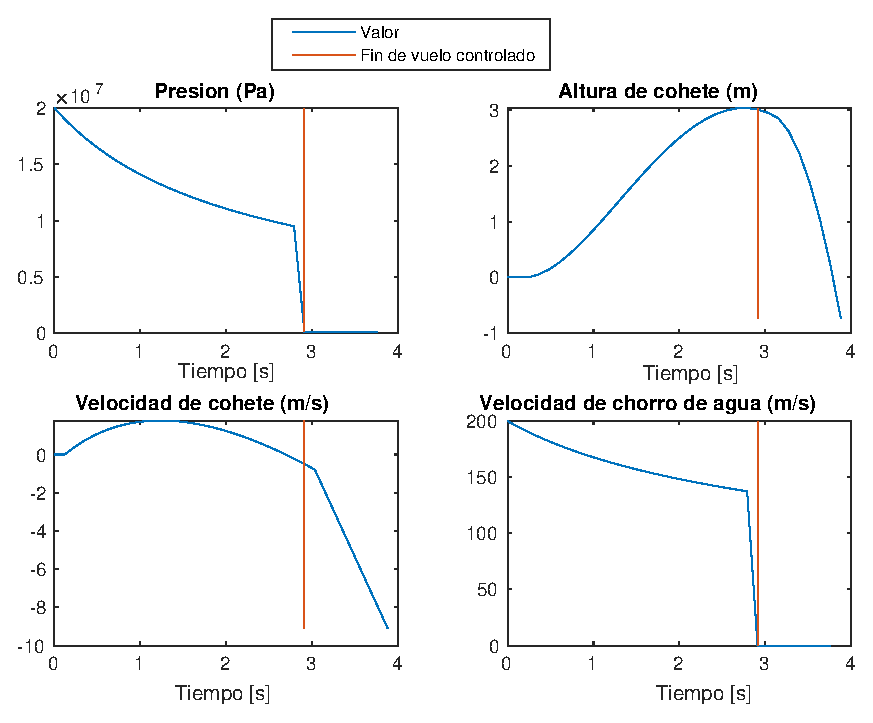
\includegraphics[width=0.8\linewidth]{fig/bottlerocket}
    \caption{Análisis preliminar para un vehículo propulsado por agua a presión. La presión es la del tanque (absoluta). El peso estructural que se utilizó fue de 10kg.}
    \label{fig:bottlerocket}
\end{figure}

Esto representa un vuelo de gran aceleración inicial, de mucha violencia, que dificulta la comprobación de sistemas en el que se tienen que tunear los parámetros de control y resolver los problemas de hardware que se vayan presentando. 

\subsection{Turbina a reacción}\label{ssec:turbina}
Se propuso la construcción de una turbina de combustible líquido, como método de propulsión
del vehículo favorable debido al excelente cociente de peso-empuje.

Esta idea se vio descartada por la pandemia que estamos atravesando (COVID19) debido a que
no teníamos acceso al taller de la institución para poder realizar en tiempo y forma el
dispositivo mecánico, que era la primer tarea inmediata a tener en banco de pruebas
asegurando su funcionamiento en optimas condiciones, para luego proseguir con el desarrollo
del vehículo y el sistema de control.


\subsection{Propulsión eléctrica}\label{ssec:propelectrica}


\begin{figure}[htb]
    \centering
    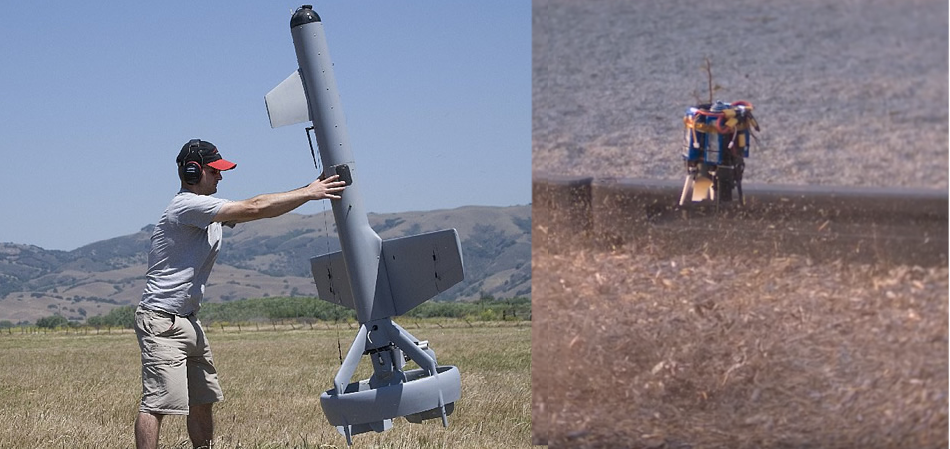
\includegraphics[width=0.8\linewidth]{fig/vbat_icarus.png}
    \caption{Dos vehículos VTVL eléctricos modernos. ``VBat'' (Izq.) e ``\href{https://hackaday.com/2018/08/31/single-rotor-drone-a-thrust-vectoring-monocopter/}{Ikarus}'' (Der.).}
    \label{fig:vbat_icarus}
\end{figure}

Luego de descartar las ideas vistas en~\ref{ssec:propAgua} y~\ref{ssec:turbina} se pasó al análisis de la incorporación de una turbina eléctrica que es un dispositivo ya existente en el mercado, no en nuestro país, pero que podría llegar a importarse. Teniendo en cuenta la pesificación del valor de los componentes en el exterior y los diversos costos asociados a la entrada al país de los mismos, se contemplo desde ese entonces la financiación privada, que la proveyó LIA Aerospace.\footnote{Agradecemos a \gls{lia} por hacerse cargo de la compra de los componentes faltantes que cayeron fuera del presupuesto necesarios para la fabricación del cohete.} 

Dadas las limitaciones de tiempo y alcance de un proyecto de la universidad se decidió por un diseño compuesto por elementos comercialmente disponibles.\footnote{\textit{Commercial off the shelf} (COTS)}

\medskip

Los vehículos VTVL eléctricos son propulsados por hélices en su mayoría y constan casi siempre de 4 o más propulsores en un arreglo simétrico y plano. Recientemente hay un interés por la construcción de vehículos de una sola hélice por la buena relación empuje--peso que tienen. Sin embargo, estos vehículos tienen sus complicaciones: 

\begin{itemize}
    \item La rotación dada al aire por la hélice causa un momento en el eje de propulsión que puede ser contrarrestado en vehículos multirrotores pero no asi en el caso de tener una sola hélice.
    \item Inclinar al rotor durante su funcionamiento causa una fuerza perpendicular a la dirección de inclinación conocido como el efecto giroscópico. 
\end{itemize}

El primer punto puede ser mitigado agregando álabes a la salida del flujo de aire por debajo del EDF para modificar el flujo y contrarestar la rotación. El segundo punto se resuelve conociendo las ecuaciones de momento angular y controlando actuadores con un sistema de control a lazo cerrado. Los sistemas vistos en la figura~\ref{fig:vbat_icarus} suelen tener la particularidad de poder ser representados con relativa facilidad usando un solo marco de referencia sobre el vehículo para calcular las ecuaciones de momento angular.

\medskip

Existen placas pre-programadas para vehículos multirrotores, pero en el caso de vehículos monorrotores de hélice fija se precisa re-programar la placa para compensar el efecto giroscópico y agregar dinámica de álabes ya que no hay software disponible aún para esta configuración. En el caso de tener una hélice móvil se suma un nivel de complejidad agregada debido al despeje de las ecuaciones de momento angular (ver sección~\ref{sec:ecuacionesRigid}). Al momento de escribir este documento aún no hay desarrollo disponible de carácter público para esta configuración.